\section{What is Flutter}

%To start with describe the high-level concept of Flutter. 
%Thereafter, a description of the low-level implementation and features of Flutter could be useful.

Flutter is a mobile \gls{ui} framework made by Google for developing Android and iOS devices\cite{flutterFAQ}. In Flutter applications  are written in a programming language called dart. Flutter translates the dart code into native arm code, for both Android and iOS.
When developing, Flutter has a "hot reload" functionally allowing for code changes to be reflected on a device or emulator without having to recompile the application first.

In Flutter all UI elements are a widget, this means that everything from a  button, to a  whole screen, which consists of multiple widgets, is a widget in it self. This gives flexibility and reusability in how widgets can be built. When working with widgets an important concept in Flutter is stateless widgets and stateful widgets. Stateless widgets are widgets that does not need to change, this could be  e.g a static description text, or a logo. Stateful widgets are useful when the widgets state needs to change in one form or the other.  An example of a stateful widget can be a text input area, where the \gls{ui} needs to reflect what is typed. Stateful widgets then helps Flutter to decide which widgets to redraw in the \gls{ui}.

\begin{figure}[h]
    \centering
    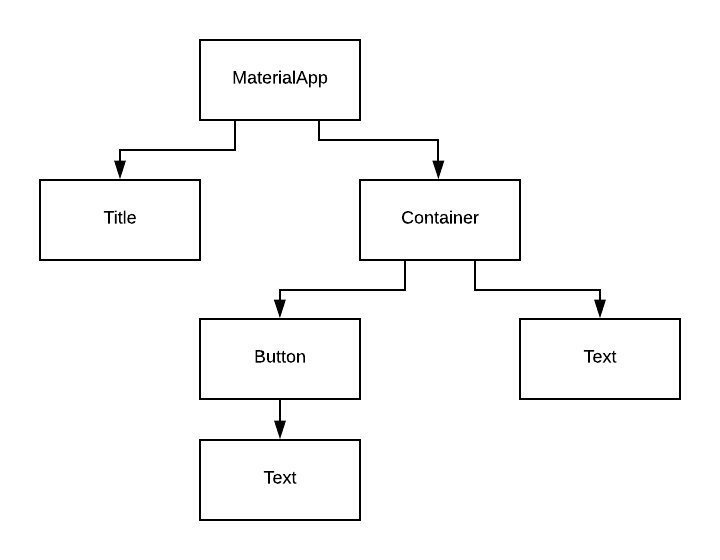
\includegraphics[width=0.8\textwidth]{figures/WidgetTree.png}
    \caption{Example of how widgets can be combined to a \textit{widget tree}. Each box is a widget, note that even text is a widget}
    \label{fig:WidgetTree}
\end{figure}

If functionality is need which is not a part of the standard Flutter libraries, a plugin can be made \cite{docker_plugins}. In Flutter a plugin is a package which contains three tings.

\begin{itemize}
    \item  Dart Api code
    \item  Android specific code
    \item  iOS specific code
\end{itemize}

A plugin then allows to write new dart functionalities, and then define what an iOS and Android implementation of the dart code looks like on each respective platform. This allows for keeping all the application code in dart code, and when extending Flutter  with new functionalities, the plugin tells Flutter how to implement the new functionality on each platform, so the dart code is free of platform specific implementation code.